\documentclass[a4paper]{article}
\usepackage[utf8x]{inputenc}
\usepackage[german,ngerman]{babel}
\usepackage[a4paper,hmargin=2cm,vmargin=3cm]{geometry}
\usepackage[hyperindex=true]{hyperref}
\usepackage{tabularx}
\usepackage{graphics}

\setlength{\headheight}{27pt} % header with two lines
\setlength{\parindent}{0pt}
\setlength{\parskip}{4pt}

\title{Bachelor-Arbeit: Protokoll Spezifikation}
\author{Christoph Peltz}

\begin{document}
\maketitle
	\begin{tabularx}{\linewidth}{|l|l|l|l|X|}
		\hline
		\textbf{Version} & \textbf{Datum} & \textbf{Autor} 	& \textbf{Status} & \textbf{Kommentar} \\
		\hline
		\hline
		1 				 & 25.02.2009 	  & Christoph Peltz & 				  & Erste Version \\
		2 				 & 01.05.2009 	  & Christoph Peltz & 				  & Korrigierung und neue Features \\
		3				 & 24.07.2009	  & Christoph Peltz &				  & Option und Advanced Drive Befehl \\
		4				 & 26.07.2009	  & Christoph Peltz &				  & Befehls-Bibliothek Nutzung\\
		\hline
	\end{tabularx}

\pagebreak
\tableofcontents
\pagebreak
	\section{Aktuelle Lage und Ziele}

	\subsection{Aktuelle Lage}

	Momentan besteht das Protokoll der Motorplatine aus einer Zusammensetzung von String-Literalen, die eine bestimmt Form haben müssen.
	Wie z.B. "d,n,n,100,100" lässt das Fahrzeug ohne PID-Korrektur fahren, die beiden Räder werden mit der Geschwindigkeit 100
	betrieben und es werden keine Trigger verwendet. Diese Form des Protokolls ist für Menschen gut lesbar und auch das Eintippen
	eines Befehles dieser Form ist sehr simpel, dies ist allerdings nicht der Fall für einen Computer, insbesondere die hier
	verwendeten Praktikumsplatinen können nicht besonders effizient mit Zeichenketten umgehen. Außerdem verbrauchen diese unnötigen
	Speicherplatz und auch dieser ist auf diesen eingebetten Systemen eine knappe Ressource mit der sehr sorgfältig umgegangen
	werden sollte. Zusätzlich wird durch die Länge eines Befehls die Geschwindigkeit mit der dieser Befehl zum einen über den Bus
	gesendet werden kann, als auch die Geschwindigkeit mit der er verarbeitet werden kann begrenzt. Denn die Befehle haben durch
	die Verwendung von Zeichenketten und die begrenzte Benutzung von den möglichen Werten eine längere Verarbeitungsdauer (BEWEIS!).

	\subsection{Ziele}

	Ein Teilziel der Bachelor-Arbeit ist das Protokoll so zu ändern, dass die Prozessoren der Platinen besser damit umgehen können.
	Das bedeutet zum einen, dass der Ansatz der Zeichenkettenrepräsentation der Befehle verworfen wird und stattdessen ein 
	Byte-orientiertes Protokoll benutzt wird das eine wesentlich höhere Informationsdichte besitzt.


	\section{Protokoll}

	\subsection{Aufbau}

	Wie bereits erwähnt ist das Protokoll Byte-orientiert, das bedeutet also dass die Informationen der Befehle keine
	lesbare Repräsentation mehr besitzen, es sind einfach eine Aneinanderreihung von Bytes. Von besonderer Wichtigkeit
	ist das erste Byte eines Befehls, im folgenden Type-Byte genannt, da es sowohl die Art des Befehles spezifiziert, als
	auch etwaige Optionen, die das Verhalten des Befehls beeinflussen oder vollkommen verändern können. Dazu ist das Type-Byte
	logisch in zwei Teile unterteilt. Die ersten vier Bit (lies least significant bits) spezifizieren einen von 16 möglichen
	Befehlen (inklusive des Reservierten Befehls 0x00, der für zukünftige Erweiterungen vorgesehen ist), die oberen vier Bit 
	(lies most significant bits) können Optionen für den ausgewählten Befehl sein. Diese Optionen reichen von Einstellungen
	für bestimmte Räder, über auswählen eines Unterbefehls bis hin zu einem völlig anderen Verhaltens des Befehles (siehe
	die Option 0xc0 des Drive-Befehls (0x03)). Alle darauf folgenden Bytes sind Parameter (mit der einen Ausnahme des
	0x00-Befehls, auch als Extended Instruction bezeichnet), deren Anzahl sich durch die Kombination von Befehl-Typ und
	Befehl-Optionen ergibt.
	Es gibt keine spezifischen Start und/oder Stop Muster, das Protokoll verlässt sich auf die ordentliche Übertragung
	der Daten und auf die korrekte Dateninhalte. Es können nur fehlerhafte Type-Bytes erkannt und abgefangen werden, dies wird
	allerdings in der Implementation zugunste der einfacheren Behandlung nur bei fehlerhaften Befehls-Typen (die unteren 4 bit) getan.
	Fehlerhafte Optionen werden ignoriert.
	Eine weitere Eigenschaft des Protokolls ist, dass ein bestimmter Befehl immer gleich viele Bytes benötigt und die Anzahl
	der Bytes nicht von den Parametern abhängt (wie es im alten Protokoll der Fall war).
	\begin{figure}[!ht]
		\centering
		\scalebox{0.3}{
			\fbox{
				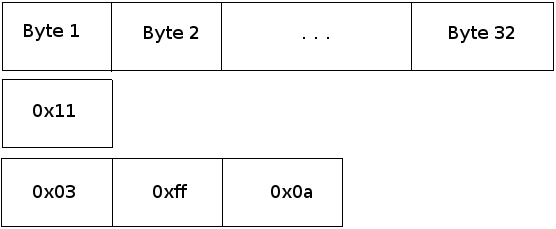
\includegraphics{Aufbau.png}
			}
		}
		\caption{Schematischer Aufbau eines Befehls und zweier Beispiele (mittleres ist ein Reset, unteres ein Fahrbefehl ohne
		Trigger mit den Geschwindigkeiten -128 und 10}
	\end{figure}

	\subsection{Extended Instruction - 0x00}

	Dieser Befehl ist für zukünftige Erweiterungen des Protokolls gedacht, falls mehr als 15 verschiedene Befehle
	benötigt werden. Wird dieser Befehl angetroffen, so werden nachfolgende Bytes als zusätzliche Type-Bytes gewertet
	und besonders behandelt.
	In der aktuellen Implementierung wird nur das erste Type-Byte eingelesen, danach gilt der Befehl als beendet. Bei der
	Ausführung des Befehls wird nichts getan, nur der Befehlsstatus auf DONE gesetzt.

	\subsection{Control - 0x01}

	Dieser Befehls ist eher eine Befehlsgattung, der sehr unterschiedliche Optionen zu Verfügung stellt. So wird der
	Befehl benutzt um das Board und die Software zu reseten, die Ausführung des Aktuellen Befehls zu stoppen, den
	nächsten Befehl in der Warteschlange zu bearbeiten, einen Fahrstopp mit aktivem Bremsen auszuführen oder einfach die
	Warteschlange zu leeren. 
	Control-Befehle können nicht in die Warteschlange eingereiht werden und es kann nur eine gleichzeitig verarbeitet werden.
	Sie umgehen die Warteschlange und werden sogar während noch laufenden Befehlen ausgeführt. Sie erhalten den frühst
	möglichen Zeitslot zur Ausführung.

	\subsection{Queue - 0x02}

	Durch diesen Befehl kann der Benutzer bestimmte Werte des Boards abfragen. Diese stellen dann Informationen
	wie z.B. die aktuelle Geschwindigkeit oder den aktuellen Befehl zu Verfügung.

	\subsection{Drive - 0x03}

	Mithilfe des Drive-Befehls werden allgemeine Fahrbefehle angenommen. Zu den Optionen zählen die Benutzung von Triggern
	auf Rad-Ebene, wie z.B. Kein Trigger, Positions-Trigger und Zeit-Trigger. Außerdem gibt es hier die Möglichkeit
	mithilfe des Differntialausgleichs sehr genau geradeaus zu fahren.

	\subsection{Advanced Drive - 0x04}

	Der Advanced-Drive-Befehl ist in erster Linie ein Drive-Befehl mit erweiterten Trigger-Bedingungen. So ist es möglich
	ein Rad entweder 100 ms oder 2000 Ticks fahren zu lassen oder aber das Rad erst dann annzuhalten, wenn es mindestens
	100 ms und 2000 Ticks gefahren ist.

	\subsection{SetPID - 0x05}

	Durch diesen Befehl ist es möglich die Parameter für eine PID-Verbesserte-Fahrt selber zu setzen und somit für sich
	anzupassen.

	\subsection{Option - 0x06}

	Dank des Option-Befehls ist es dem Benutzer möglich Werte für bestimmte Verhaltenskritische Variablen während des
	Betriebs zu verändern.

	\subsection{0x07 - 0x0f}

	Diese Befehlscodes sind bisher nicht vergeben.


	\section{Befehlsreferenz}

	\subsection{Extended Instruction - 0x00}

	Bisher werden Befehle mit diesem Code werden nach einem Byte abgebrochen und in die Queue gestellt. Es existiert noch
	keine Anwendung für diese Befehlsgattung.

	\subsection{Control - 0x01}

	\begin{tabularx}{\linewidth}{|l|l|X|}
		\hline
		\textbf{Option} & \textbf{Bitmaske} & \textbf{Beschreibung} \\
		\hline
		\hline
		Reset 			& 0x10 				& Resetet die Hardware \\
		\hline
		Stop Queue		& 0x20				& Der Aktuelle Befehl wird verworfen. Queue wird angehalten, aber nicht verworfen. \\
		\hline
		Continue Queue	& 0x30				& Der nächste Befehl in der Queue wird ausgeführt. \\
		\hline
		Clear Queue		& 0x40				& Die Warteschlange wird gelöscht. \\
		\hline
		Stop Drive		& 0x50				& Befehl wird angehalten, Fahrzeug geht zum aktiven Bremsen über. \\
		\hline
	\end{tabularx}

	Um auf das richtige Befehlsbyte zu kommen muss die Option mit dem Befehl verundet werden. Als Beispiel dient hier das Löschen
	der Queue: 0x40 \& 0x01 = 0x41. Dies gilt für alle Befehle hier.
	Der Control-Befehl hat keine Parameter und ist damit konstant 1 Byte lang. Außerdem umgehet dieser Befehl die Warteschlange,
	wird also sofort ausgeführt, auch während noch ein anderer Befehl bearbeitet wird.

	\subsection{Query - 0x02}

	\begin{tabularx}{\linewidth}{|l|l|X|}
		\hline
		\textbf{Bitmaske} & \textbf{Beschreibung} & \textbf{Antwortlänge} \\
		\hline
		\hline
		0x10 				& Geschwindigkeit des linken Rades & 1 \\
		\hline
		0x20				& Geschwindigkeit des rechten Rades & 1 \\
		\hline
		0x30				& Anzahl der Befehl in der Queue & 1 \\
		\hline
		0x40				& Aktueller Befehl & 2 - 33 (siehe Text) \\
		\hline
	\end{tabularx}
	
	Der Query-Befehl ist immer nur ein Byte lang, in den oberen 4 bit wird spezifiziert welche Informationen man haben möchte.
	Welche zur Verfügung stehen und welche Bitmaske man dafür verwenden muss, wird aus der obigen Tabelle entnommen. Es kann immer
	nur ein Wert per Befehl abgefragt werden. Die Antwort auf solch eine Anfrage hat eine variable Länge, die ebenfalls aus
	der Tabelle entnommen werden kann (sie ist in Byte angegeben).
	Bei der Antwort mit dem Aktuellen Befehl gilt zu beachten, dass zweimal von der Platine gelesen werden muss. Die erste
	Antwort ist immer 1 Byte lang und gibt an wie lang die zweite Antwort sein wird. Diese hält dann den eigentlichen Befehl.

	\subsection{Drive - 0x03}

	Beim Drive Befehl sind die vier Optionsbits in zweimal zwei Bit unterteilt, die jeweils für ein Rad den Trigger angeben.

	\begin{tabularx}{\linewidth}{|l|l|l|X|}
		\hline
		\textbf{Option} & \textbf{Bitmaske linkes Rad} & \textbf{Bitmaske rechtes Rad} & \textbf{Beschreibung} \\
		\hline
		\hline
		Kein Trigger	& 0x00						   & 0x00						   & Endlosfahrt \\
		\hline
		Zeit Trigger	& 0x10						   & 0x40						   & zeitlich Begrenzte Fahrt\\
		\hline
		Positions Trigger & 0x20					   & 0x80						   & Fährt eine bestimmte Strecke \\
		\hline
	\end{tabularx}
	
	Hier müssen für beide Räder eine Options ausgewählt werden und zusammen auf den Befehl geundet werden. Beispiel linkes
	Rad benutzt einen Zeit Trigger, das rechte einen Positionstrigger: 0x10 | 0x80 | 0x03 = 0x93.
	Der Befehl erwartet mindestens zwei Parameter, die jeweils ein Byte lang sind und die Geschwindigkeit vom linken und
	vom rechten Rad angeben.

	\begin{tabularx}{\linewidth}{|l|l|l|X|}
		\hline
		\textbf{Byte Anzahl} & \textbf{Option} & \textbf{Wertebereich} & \textbf{Beschreibung} \\
		\hline
		\hline
		1					 & - & -128 bis 127 & Geschwindigkeit des linken Rades \\
		\hline
		1					 & - & -128 bis 127 & Geschwindigkeit des rechten Rades\\
		\hline
		2					 & Zeit Trigger & 0 bis 65535 &  Anzahl der ms die das linke Rad fährt\\
		\hline
		2					 & Positions Trigger & 0 bis 65535 &  Anzahl der Ticks die das linke Rad fährt\\
		\hline
		2					 & Zeit Trigger & 0 bis 65535 &  Anzahl der ms die das rechte Rad fährt\\
		\hline
		2					 & Positions Trigger & 0 bis 65535 &  Anzahl der Ticks die das rechte Rad fährt\\
		\hline
	\end{tabularx}
	
	Die Parameter werden in der Reihenfolge erwartet die hier angegeben wurde wobei die Zeit und Positionsparameter nur
	angegeben werden müssen wenn für des entsprechende Rad dies auch in den Optionen aktiviert wurde.
	Die Minimale Länge beläuft sich damit auf 3 Byte (1 Byte Kommando + 2 Byte für die Geschwindigkeiten) und die
	Maximale auf 7 Byte (1 Byte Kommando + 2 Byte Geschwindigkeit + 2*2 Byte für Trigger-Werte pro Rad).

	Es gibt noch einen speziellen Fahrmodus: Fahren mit Differentialausgleich. Dieser wird aktiviert wenn im Befehlsbyte
	die Bitmaske 0x30 benutzt wird. Die Trigger Bitmasken für das rechte Rad (siehe Tabelle) gelten dann für beide Räder.
	Folgend auf das Befehlsbyte tut dann ein Geschwindigkeitsbyte sowie, falls erforderlich, 2 Bytes für den ausgewählten
	Trigger. Die Minimale Länge beläuft sich hier auf 2 Byte, die Maximale auf 4.

	Wenn die Bitmaske 0xc0 auf dem Befehlsbyte genutzt wird, kann der relative Differentialwert für die Fahrt eingestellt
	werden. Ein Wert gleich 0 setzt den Wert auf 0. Von 0 verschiedene Werte werden auf den aktuellen Differentialwert
	addiert. Der Differntialwert darf einen wert zwischen -32768 bis 32767. Die Länge beträgt immer 3 Byte.

	\subsection{Advanced Drive - 0x04}

	Ist identisch zu dem Drive Befehl, bis auf folgende Ausnahmen:
	
	\begin{tabularx}{\linewidth}{|l|l|l|X|}
		\hline
		\textbf{Option} & \textbf{Bitmaske linkes Rad} & \textbf{Bitmaske rechtes Rad} & \textbf{Beschreibung} \\
		\hline
		\hline
		Kein Trigger				& 0x00						   & 0x00						   & Endlosfahrt \\
		\hline
		Zeit ODER Position Trigger	& 0x10						   & 0x40						   & zeitlich Begrenzte Fahrt\\
		\hline
		Zeit UND Positions Trigger  & 0x20						   & 0x80						   & Fährt eine bestimmte Strecke \\
		\hline
	\end{tabularx}

	Außerdem sind die Bitmasken 0x30 und 0xc0 hier ungültig. Der "Zeit ODER Position"-Trigger bewirkt, dass das Rad angehalten
	wird, wenn einer der beiden Trigger erreicht wurde. Analog bewirkt der "Zeit UND Position"-Trigger, dass das Rad
	beide Trigger erfüllen muss, bevor das Rad angehalten wird. Dadurch, dass jetzt zwei Trigger gleichzeitig angegeben werden
	pro Rad ist wichtig zu wissen, wo die Bytes hinkommen müssen. Dies zeigt die folgende Illustration:
	\begin{figure}[!ht]
		\centering
		\scalebox{1.0}{
				
\includegraphics{advanced_drive_instruction.png}
		}
		\caption{Ein Advanced-Drive-Befehl mit Zeit ODER Position Trigger für beide Räder (daher die 0x54)}
	\end{figure}
	Wenn kein Trigger verwendet wird, benötigt der Befehl 3 Byte, wenn für beide Räder Trigger verwendet werden sind es im
	maximal Fall 11 Byte.
	

	\subsection{SetPID - 0x05}

	Mithilfe dieses Befehls können die Reglergrößen für den PID-Regler eingestellt werden.

	\begin{tabularx}{\linewidth}{|l|l|l|X|}
		\hline
		\textbf{Byte Anzahl} & \textbf{Position} & \textbf{Wertebereich} & \textbf{Beschreibung} \\
		\hline
		\hline
		2					 & 1 & -32768 bis 32767 & Proportinaler Faktor\\
		\hline
		2					 & 2 & -32768 bis 32767 & Integraler Faktor\\
		\hline
		2					 & 3 & -32768 bis 32767 & Differentieller Faktor\\
		\hline
		2					 & 4 & -32768 bis 32767 & Maximale Fehlersummen Modifikator\\
		\hline
	\end{tabularx}

	Im Befehlsbyte muss außerdem einkodiert werden für welches Rad die Parameter gesetzt werden.

	\begin{tabularx}{\linewidth}{|l|X|}
		\hline
		\textbf{Option} & \textbf{Bitmaske} \\
		\hline
		\hline
		Linkes Rad	& 0x00 \\
		\hline
		Rechtes Rad	& 0x10 \\
		\hline
		Beide Räder & 0x20 \\
		\hline
	\end{tabularx}

	Die Länge des Befehls beträgt immer 9 Byte.

	\subsection{Option - 0x06}

	Der Option-Befehl dient dazu Verhaltenskritische Variablen während des Betriebs zu verändern.
	Die oberen 4 Bit des Befehlsbytes geben an, welche Variable gesetzt werden soll. Anzumerken ist,
	dass 0x06 an sich, also die oberen 4 Bit gleich 0, reserviert ist für zukünftige Erweiterungen.

	\begin{tabularx}{\linewidth}{|l|l|l|X|}
		\hline
		\textbf{Bitmaske} & \textbf{Default} & \textbf{Wertebereich (Bytes)} & \textbf{Beschreibung} \\
		\hline
		\hline
		0x10 & 40 & 1 bis 127 (1) & Der Geschwindigkeitswert, der beim aktiven Bremsen benutzt wird. \\
		\hline
		0x20 & 1 & 0 oder 1 (1) & Switch zum aktivieren des aktiven Bremsen. Eine 1 bedeutet, dass das Bremsen aktiviert ist. \\
		\hline
		0x30 & 1 & 0 oder 1 (1) & Switch zum aktivieren des aktiven Bremsens, eines Rades, das bereits seinen Trigger erreicht hat, das andere aber noch weiterfährt. \\
		\hline
		0x40 & 1 & 0 oder 1 (1) & Switch zum aktivieren des aktiven Bremsens, wenn kein Befehl bearbeitet wird. \\
		\hline
	\end{tabularx}

	0x20 kann zum einfachen an- und ausschalten des Aktiven Bremsens verwendet werden,
	die 0x30 und 0x40 Varianten sind für die Einschränkung des Aktiven Bremsens, wenn es
	aktiviert ist, verantwortlich. 0x10 wird, wenn ein Wert außerhalb des Wertebereichs
	angegeben wird, den default-Wert benutzen. Momentan sind alle Option-Befehle 2 Byte lang.
	
	\section{Verwendung der Befehls-Bibliothek}
	
	Die Befehls-Bibliothek ist optional und klein. Sie dient hauptsächlich dazu das Senden von Befehlen an
	die Motorplatine zu vereinfachen. Ohne die Bibliothek muss der Benutzer selber alle Felder eines Arrays
	korrekt setzen und sie selber senden. Die Bibliothek hingegen sellt eine große Menge an defines bereit,
	die das spätere lesen des Codes vereinfachen, sowie einige Funktionen, die das füllen der Parameter
	kurz und übersichtlich hält. Natürlich hat dies einen geringen Overhead zur Folge (mindestens wegen der
	Funktionsaufrufe).
	Um einen Befehl mit der Bibliothek zu erstellen und abzusenden sind folgende folgene Schritte durchzuführen:
	\begin{enumerate}
		\item Erstellen einer Variable vom Typ order\_t
		\item Initialisieren dieser Variable mit order\_init(order\_t)
		\item Einstellen des Befehlstypes mit order\_set\_type(order\_t, type) (Hierfür gibt es eine Menge an defines
			um diesen Aufruf kurz und informativ zu halten)
		\item Setzen, wenn nötig, der Parameter für den Befehl, mithilfe von order\_add\_params(order\_t, format, param1, ..., paramN)
		\item Senden des Befehls an die Platine mithilfe von order\_send(order\_t), order\_send\_and\_recv(order\_t) oder
			order\_send\_and\_recv\_co(order\_t).
	\end{enumerate}
	Wichtige Besonderheiten sind, dass der Typ order\_t, zwar größenteils identisch mit dem auf der Platine verwendete
	Typ ist, statt einer status-Variablen jetzt eine pos-Variable hat, die {\em nur intern verwendet} werden darf.
	Sie speichert die Schreibposition sowie die länge des Befehls. Das große data Array musste hier in dat umbenannt
	werden, da data ein reserviertes Wort unter Keil ist. Das erste Feld in dem dat Array speichert die Adresse der
	Platine und wird während order\_init(order\_t) gesetzt. Ab dem zweiten Feld des dat Array residieren hier nur die
	Befehlsdaten.
	Mit order\_set\_type(order\_t, type) wird der Typ des Befehls gesetzt, das bedeutet, das erste Byte des Befehls auch
	Befehlsbyte genannt. Für jeden validen Typ, das schließt auch alle Optionen mit ein, gibt es ein define, welches man
	hierfür verwenden kann.
	Die Funktion order\_add\_params(order\_t, format, param1, .., paramN) hat eine variable Anzahl an Parametern. Die
	Anzahl der Parameter und deren Typen wird durch den format-String festgelegt. Dieser besteht aus einer Kombination
	aus 1en und 2en. Die 1en bedeuten ein 1-Byte Parameter (int8\_t oder äquivalent) wobei die 2en ein 2-Byte
	Parameter bedeuten (int16\_t oder äquivalent). Sie werden in der Reihenfolge in der sie angegeben wurden auch erwartet
	und eingefügt. Beispiel: "1121" würde aussagen, dass zwei 1-Byte Parameter, dann ein 2-Byte Parameter, gefolgt von
	einem weiteren 1-Byte Parameter erwartet wird.
	Wenn der Befehl nun zur Zufriedenheit konstruiert wurde, kann er mit einem der drei send-Funktionen gesendet werden.
	Wichtig ist hier die Richtige auszuwählen. Dabei gilt, wird keine Antwort auf den Befehl erwartet (der Großteil der
	Befehle), dann wird order\_send(order\_t) benutzt. Die Funktion gibt die Anzahl der gesendeten Bytes zurück.
	Falls der Befehl eine Antwort provoziert (wie die query-Befehle), dann wird order\_send\_and\_recv(order\_t) benutzt.
	Dieser wird den Befehl senden und an die Stelle der Alten Befehlsdaten (also ab dem zweiten Feld) die Antwort einlesen.
	Außerdem gibt der Befehl die Anzahl der gelesenen Bytes zurück. (pos wird nicht korrekt gesetzt).
	Es gibt noch einen Befehl zum Senden und Empfangen, das ist der order\_send\_and\_recv\_co(order\_t). Dieser muss
	benutzt werden, wenn die Antwort der Platine eine variable Länge hat (so wie die Antwort auf den Query nach dem
	aktuellen Befehl (current order) von dem der Befehl auch seinen Namen ableitet. Auch dieser Befehl gibt die Anzahl
	der empfangenen Bytes zurück und speichert die empfangenen Daten ab dem zweiten Feld des dat-Arrays.

	\section{Befehlsbeispiele}

	\subsection{Control - 0x01}
	
	Reset: 0x01 OR 0x10 = 0x11\\
	Stop Drive: 0x01 OR 0x50 = 0x51

	\subsection{Query - 0x02}
	Anzahl der Befehle: 0x02 OR 0x30 = 0x32\\
	Antwort (unter der Annahme, dass 5 befehle in der Queue sind): 0x05

	\subsection{Drive - 0x03}
	Die Geschwindigkeit des linken Rades soll 100 sein, die des rechten -50. Das linke Rad soll einen Zeit- und das
	rechte einen Positionstrigger verwenden. Die Zeit soll 500 betragen, die Position 10000.\\
	Erstes Byte: 0x03 OR 0x10 OR 0x80 = 0x93\\
	Gesamte Befehl: 0x93 0x64 0xce 0x01 0xf4 0x27 0x10

\end{document}
